\documentclass[a4paper,10pt, leqno]{article}
\usepackage[utf8]{inputenc}
\usepackage[hmargin=3cm,vmargin=2cm]{geometry}
\usepackage[bulgarian]{babel}
\newcommand{\HRule}{\rule{\linewidth}{0.5mm}}
\usepackage{xspace}
\usepackage{amsmath}
\usepackage{verbatim}
\usepackage[unicode]{hyperref}
\hypersetup{
colorlinks=true,
linkcolor=black,
pdftitle={Проект по ASP програминране},
pdfauthor={Емил Станчев},
pdfsubject={Бази от данни},
pdfcreator={Емил Станчев}
}
\usepackage{yfonts}
\usepackage{amsthm}
\usepackage {amssymb}
\usepackage{graphicx}
% for source code inclusion
\usepackage{listings}
\renewcommand{\lstlistingname}{\bfseries Файл}
\lstset{caption=\lstname, numbers=left, numberstyle=\tiny}
\lstset{keywordstyle=\bfseries}
\lstset{commentstyle=\color{darkgray}}
% \\lstset{ language=Matlab, caption=\\lstname, numbers=left, numberstyle=\\tiny}
% \\lstset{keywordstyle=\\bfseries}
% \\lstset{commentstyle=\\color{darkgray}}
%\lstset{frame=T}
\newcommand{\asp}{ASP\xspace}
\newcommand{\figref}[1] {Фигура \ref{#1}}
\newcommand{\term}[1] {\textsl{#1}}
\newcommand{\tab}[1] {\textbf{#1}}
\newcommand{\col}[1] {\textbf{#1}}
\newcommand{\File}[1] {\texttt{#1}}

\begin{document}

% TITLE PAGE
\begin{titlepage}
    \begin{center}
        \textsc{СУ ``Св. Климент Охридски''\\
        Факултет по математика и информатика
        }\\[5cm]

        \textsc{\large Проект по \\
        ASP програмиране
        }\\[0.5cm]
        \HRule \\[0.4cm]
        { \Large \bfseries Online билетна каса за спортни прояви
        }\\[0.4cm]
        \HRule \\[6cm]
        \begin{minipage}{0.49\textwidth}
            \begin{flushleft} \large
                \emph{Автор:}\\
                Емил Станчев,\\
                \small ф.н.71100
            \end{flushleft}
        \end{minipage}
        \begin{minipage}{0.49\textwidth}
            \begin{flushright} \large
                \emph{Преподавател:} \\
                доц. д-р Павел Павлов
            \end{flushright}
        \end{minipage}
        \vfill
        {\large \today}
    \end{center}
\end{titlepage}

\tableofcontents
\newpage

\section{Задание}
Проектът създава онлайн система за онлайн билетна каса за
спортни прояви. Проектът трябва да обслужва два типа
потребители - администратор и клиент. Организацията на работата
на касата предполага, че заявката за билет от клиента става
дистанционно, а доставката на билета се извършва от
специализирана куриерска служба.
Администраторите отговарят за поддържането и контрола на
данните. Добавят спортна проява с дата, начален/краен час,
място на провеждане, брой билети. Променят броя билети при
продажба. Преглеждат заявки за закупуване на билети и извършват
продажбата им. Актуализират данни за спортна проява. Изтриват
спортна проява. Правят справки колко свободни билети има за
дадена проява, колко са продадените билети за проява, за месец.
Клиентът разглежда списък със спортни прояви. Възможност за
търсене от дата до дата, по тип на спортна проява и др. При
избор на спортна проява вижда пълен списък с данни за проявата.
Има възможност да направи заявка за закупуване на един или
повече билета за спортната проява. Може да види сумата, която
трябва да заплати. Заявката се изпраща до администратора, който
при налични места извършва продажбата. 

\section{Реализация}
\subsection{База от данни}
За проекта е използвана системата за управление на бази от данни \term{PostgreSQL} с официалния \term{ODBC} драйвер.
Системата е настроена за работа с \term{UTF-8} кодиране на символите. На следващата фигура е показан релационният
модел на базата от данни.

\begin{figure}
    \centering
    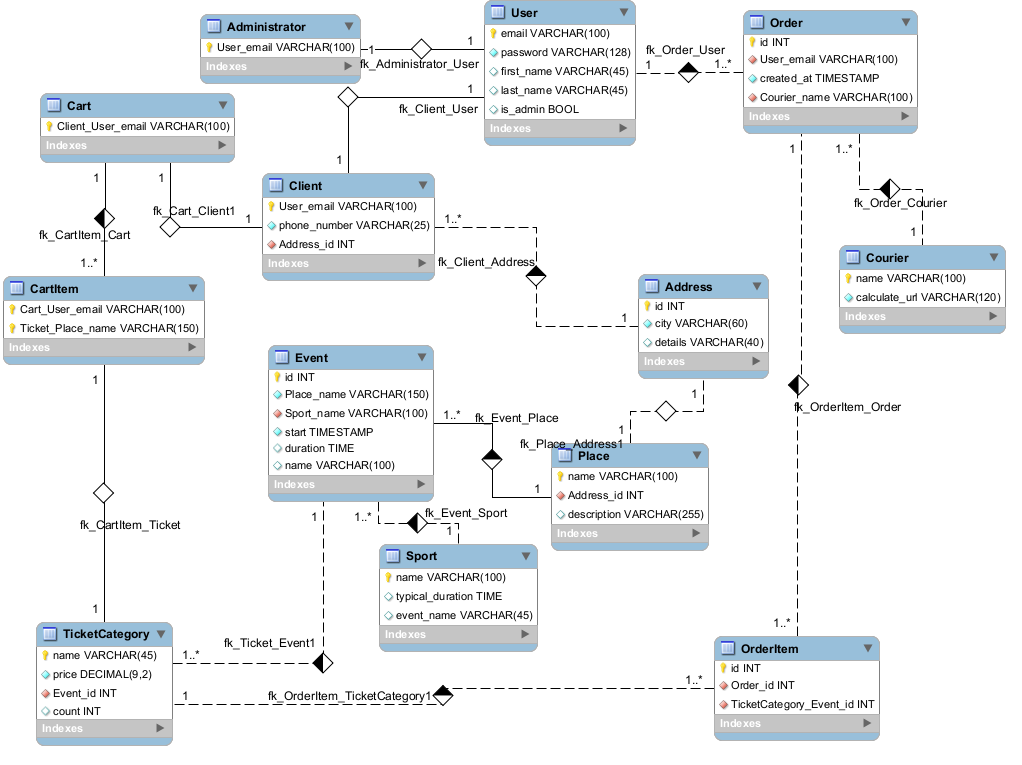
\includegraphics[width=15cm]{../database/relational_model.png}
    \label{fig:r}
    \caption{Релационен модел}
\end{figure}

По-долу следват подробности за таблиците и тяхното значение:

\begin{description}
    \item[\tab{User}]
        Потребител на системата, за когото се пази информация за собствено и фамилно име (\col{first\_name} и \col{last\_name}),
        парола (\col{password}). Паролите се пазят като хеширани стрингове с \term{MD5} алгоритъм, смесени със „сол“. Всяка парола
        е най-малко 5 символа. Таблицата \tab{User} представлява абстрактен клас - инстанции на \tab{User} не могат да се създават -
        само инстанции на „наследниците“ \tab{Administrator} и \tab{Client}.
        Първичен ключ на тази таблица е \tab{email}.
        Проверката дали даден потребител е администратор се извършва като се провери колоната \col{is\_admin}. Стойността на \col{is\_admin}
        се променя чрез тригер, който се активира при прибавянето на нов администратор (ред в таблицата \tab{Administrator}).
    \item[\tab{Client}]
        Клиент на системата. Тази таблица е в отношение 1 към 0..1 с \tab{User}. Поради тази причина първичният ключ на \tab{Client} е
        външният ключ към таблицата \tab{User} - \tab{User\_email}. Всеки клиент има освен „наследените“ атрибути на \tab{User} и
        телефонен номер (\col{phone\_number}) и външен ключ към адрес \tab{Address}.
    \item[\tab{Address}]
        Таблица с адреси. Тези адреси могат да са както на клиенти, така и на спортни съоръжения. Колоната \col{city} указва града,
        а \col{details} съхранява останалата част от адреса.
    \item[\tab{Place}]
        Таблица със спортни съоръжения. Всяко спортно съоръжение има име (\col{name}) и външен ключ към адрес (\col{Address\_id}), както и
        кратко текстово описание. Първичен ключ е \col{name}.
    \item[\tab{Event}]
        Спортна проява. Всяка спортна проява се случва на дадено спортно съорежение (външен ключ \col{Place\_name}), и включва даден
        вид спорт (външен ключ \col{Sport\_name}). Всяка проява има начален час (\col{start}) и продължителност (\col{duration}). Ако 
        продължителността не е зададена, стойността по подразбиране е \texttt{NULL}. Ако стойността е \texttt{NULL}, за продължителност
        на събитието се счита типичната продължителност на асоциирания спорт (\col{typical\_duartion} колоната на таблицата \col{Sport}).
        Първичният ключ е сурогатен (\col{id}).
    \item[\tab{Sport}]
        Даден вид спорт. Ключ е името (\col{name}). \col{typical\_duration} е типичната продължителност за даден вид спорт (например, $90$ минути
        за футболен мач); тази стойност се използва за продължителност на спортната проява, ако такава не е зададена.
    \item[\tab{TicketCategory}]
        Категория билети. Всяка спортна проява има една или повече категории билети, всяка от които има име (\col{name}), дадена цена (\col{price}),
        и налична бройка билети от тази категория (\col{count}). Например, можем да имаме категория с име „Сектор А“ с цена на билета $12$лв. и
        налични 5000 билета.
    \item[\tab{Cart}]
        Таблица, съхраняваща количката на клиент. Всяка количка е асоциирана с точно един клиент (\col{Client\_User\_email}).
    \item[\tab{CartItem}]
        Таблица, съдържаща информация за артикулите в количката на даден клиент. Всеки артикул представлява един или повече
        билети от дадена категория за дадена спортна проява (външен ключ \col{TicketCategory\_name}). Всеки артикул има и съответна
        бройка билети (\col{count}). Например, „3 билета за сектор А на мача Левски - Славия“.
    \item[\tab{Order}]
        Представлява завършена поръчка. Състои се от артикули (\tab{OrderItem}), и има асоцииран куриер (\tab{Courier}).
    \item[\tab{OrderItem}]
        Представлява артикул от завършена поръчка. Аналогично с артикул в количката.
    \item[\tab{Courier}]
        Всеки куриер има име (\col{name}) и \col{calculate\_url}, което е хипервръзка към сайта на куриера за изчисляване на цената.
        Тази връзка се появява при избора на куриер от клиента.
\end{description}

\subsection{Приложение}
Скриптовете на приложението са реализирани с \term{JScript}, който трябва да се конфигурира като скриптов език
по подразбиране на сървъра, защото \textbf{не е указано}

\begin{verbatim}
<% @LANGUAGE=JScript %>
\end{verbatim}
изрично във всеки \texttt{ASP} файл.
Списъкът с файлове в проекта и тяхното предназначение е показан по-долу.
Повечето от скриптовете са реализирани така, че при \term{GET} заявка те показват страница, която обикновено включва форма
за попълване, а при \term{POST} заявка изпълняват съответното действие.
Например, \File{admin/event.asp} показва нова форма на администратора при \term{GET} заявка, а при \term{POST} заявка от администратора
извършва запис в базата данни след съответната валидация.

\subsubsection{Помощни скриптове}
\begin{description}
    \item[\File{db/db.inc}] Файл, съдържащ \texttt{Javascript}-класове за базата от данни.
        Създава се един метаклас, представляващ таблица в база от данни,
        след което от него се създават класове за всяка таблица. В резултат имаме \textbf{следните класове}:
        \begin{itemize}
            \item \tab{User}
            \item \tab{Place}
            \item \tab{Sport, и т.н.}
        \end{itemize}
        Всеки от тези класове играе ролята на \textit{модел} (в смисъла, определен от \texttt{MVC} архитектурата).
        Тоест всеки клас представлява интерфейс от високо ниво към базата от данни. Всяка колона на таблица 
        от базата данни съответства на поле на обект, т.е. реализиран е прост \texttt{ORM (Object-Relational Mapper)}.
        Някои от методите са изброени по-долу. \texttt{Model} представялва произволен клас, представляващ таблица от базата данни.
        \texttt{model\_obj} представлява инстанция на \texttt{Model}.

        \begin{description}
            \item[\texttt{model\_obj.save()}] Запазва в базата от данни запис, съответстващ на \texttt{user\_obj}. Ако
                \texttt{user\_obj} представлява съществуващ запис, то се извършва \texttt{UPDATE} заявка, в противен случай
                се извършва \texttt{INSERT}. Тук се извършва и всичката валидация на данните, преди да се запази.
                % \\item[\\texttt{user\\_obj.is\\_valid()}] Връща \\texttt{true} или \\texttt{false} в зависимост от това дали
                % обектът е валиден (дали данните в полетата му са валидни).
                \item[\texttt{Model.primary\_keys}] Статичен атрибут, съдържа списък от първичните ключове. Използва се от \texttt{save} метода,
                    за да се определи дали обектът съществува като ред в таблицата, за да се направи съответно \texttt{UPDATE} или \texttt{INSERT} заявка.

                \item[\texttt{model\_obj.delete()}] Изпълнява \texttt{DELETE} заявка.
                \item[\texttt{Model.all(filter, opts)}] Статичен метод, който връща потребители като масив от обекти на класа \texttt{User}.
                    \texttt{filter} е асоциативен масив, който указва какво да се включив \texttt{WHERE} клаузата.
                    \texttt{opts} е асоциативен масив, който съдържа други опции (например, ако \texttt{opts['or']} е \texttt{true},
                    в \texttt{WHERE} клаузата се използва \texttt{OR} вместо \texttt{AND}.
                    Например, ако \texttt{Model=User}
\begin{verbatim}
User.all({'email': 'ivan@mail.bg', 'email': 'georgi@mail.bg'},
{'or': true});
\end{verbatim}
                    изпълнява заявката:
\begin{verbatim}
select * from "User"
where email='ivan@mail.bg' OR email='georgi@mail.bg';
\end{verbatim}
                \item[\texttt{Model.count(filter, opts)}] Статичен метод, връща брой записи.
                \item[\texttt{Model.find(where\_string)}] Статичен метод, който изпълнява следната заявка
\begin{verbatim}
select * from "Model" where <where_string>;
\end{verbatim}
                \item[\texttt{Model.exists(attributes)}] Проверява дали съществува ред с дадените атрибути.
            \end{description}

            Горните методи се поддържат от всички класове, съответстващи на таблици от базата данни, тъй като тези класове
            са създадени от един общ метаклас.

            Освен това този файл съдържа клас \texttt{DBConnection}, който енкапсулира връзката с базата от данни.
            Например:

\begin{verbatim}
dbc = new DBConnection('PostgreSQL35W',
'SET search_path TO tickets;');
dbc.execute('select * from "Event"');
dbc.table_names();
\end{verbatim}

            В горния пример създаваме нов обект, представляващ връзка към базата данни.
            Първият аргумент на конструктора е \texttt{dsn} идентификатора на базата от данни, който
            е зададен в \texttt{Data Sources} настройките на сървъра. Вторият аргумент е заявка, която да се изпълни при стартирането
            на връзката, в този случай пътя за търсене става схемата \tab{tickets}.

            Методът \texttt{execute} просто делегира към съответния метод на \texttt{ADOConnection}, но връща масив от обекти вместо
            \texttt{recordset}.

            Методът \texttt{table\_names} връща имената на таблиците в базата от данни.

        \item[\File{models.inc}]
            Създава инстанции на моделите за всяка от таблиците в базата данни и инициализира връзка с базата от данни:
            \lstinputlisting{models.inc}
            \renewcommand{\lstlistingname}{\bfseries Файл}
        \item[\File{util.inc}]
            Помощни функции за работа с масиви, стрингове и други. Например:
            \begin{description}
                \item[\texttt{function map(array, lambda)}]
                    Връща нов масив, който е резултат от прилагането на функцията \texttt{lambda} върху всеки елемент на масива \texttt{array}.
                \item[\texttt{function filter(array, lambda)}]
                    Връща нов масив, който се състои само от елментите на \texttt{array}, за които \texttt{lambda} връща \texttt{true}-стойност.
            \end{description}
        \item[\File{md5.inc}]
            Файл, в който е дефинирана функция, която хешира с \term{MD5} алгоритъм. Използва се при работа с пароли.

    \end{description}


    \subsubsection{Обща част}
    \begin{description}
        \item[\File{default.asp}]
            Началната страница на приложението. Показва се списък от предстоящи прояви, за които има налични билети.
        \item[\File{login.asp}]
            Това е страницата за вписване.
        \item[\File{logout.asp}]
            Изчиства се сесията и потребителят се отписва (ако не е вписан, се пренасочва към \File{login.asp}).
        \item[\File{search.asp?from=<fd>\&to=<td>\&sport=<s>\&city=<c>}]
            Търсене на проява по различни критерии.
    \end{description}

    \subsubsection{Администраторска част}
    \begin{description}
        \item[\File{admin/admin\_required.inc}]
            Скриптът в този файл проверява дали текущият потребител е администратор (използвайки атрибута \col{is\_admin} на \tab{User}).
            Ако не е администратор, то той се пренасочва към страницата
            за вписване \File{login.asp}, ако не е вписан; ако пък е вписан, се пренасочва към началната страница \File{default.asp}.
            Този файл се включва с \texttt{\#include} директива във всички файлове от директорията \File{admin/}.
        \item[\File{admin/default.asp}]
            Началната страница на администраторската част. Показва се списък от прояви, потребители и настройки.
            Администраторът получава възможност да редактира всички обекти, които се показват.
        \item[\File{admin/event.asp?id=<id>}]
            Страница за редактиране на проява. Показва се форма за въвеждане на данни за проявата с \texttt{id=<id>} и категория билети и цени.
            Ако \term{HTTP} параметърът \texttt{id} не е зададен, се отваря форма за въвеждане на нова проява.
        \item[\File{admin/place.asp?name=<name>}]
            Страница за редактиране на спортни съоръжения. Показва се форма за редактиране на мястото с \texttt{name=<name>}.
            Ако \term{HTTP} параметърът \texttt{name} не е зададен, се отваря форма за въвеждане на ново спортно съорежение.
        \item[\File{admin/client.asp?email=<email>}]
            Страница за редактиране на клиента, за който \texttt{email=<email>}.
            Всичката информация за клиента е налична и разрешена за редактиране.
    \end{description}

    \subsection{Клиентска част}
    \begin{description}
        \item[\File{client\_required.inc}]
            Проверява дали потребителят е клиент. Ако не е и е вписан като администратор, се пренасочва към \File{admin/default.asp}.
            Ако пък въобще не е вписан, се пренасочва към \File{default.asp}.
        \item[\File{profile.asp}]
            Редакция на потребителския профил.
        \item[\File{cart.asp}]
            Количката на потребителя.
            При \texttt{POST} заявка се прибавя нов артикул.
        \item[\File{order.asp}]
            Завършване на поръчката след избор на куриер и преглед на артикулите.
        \item[\File{event.asp?id=<id>}]
            Подробности за дадено събитие.
        \item[\File{history.asp}]
            История на поръчките на клиента.
    \end{description}

    \end{document}
